\Chapter{Tervezés}

% TODO: Adatbázis sémájának a definíciója.

% TODO: Az architektúra bemutatása, hogy hol milyen technológia került felhasználásra. (A szokásos szerver-kliens kialakítás néhány egyedi dologgal.)

% TODO: Az alkalmazás felépítéséről UML ábrák. Minél részletesebben bemutatva, hogy minek kellene majd elkészülnie.

%DevTools Maven-ben arra használható, hogy ne kelljen minden módosítás után újrafordítanunk, hanem ha megváltozott a forráskód akkor megteszi helyettünk az IDE.
 
Az alkalmazástervezési fázist megelőzte a technológiai tervezés fázisa. A kronológiai sorrendet betartva a felhasználandó technológia bemutatásával kezdem ezt a fejezetet.  

\begin{comment}{Az időrendi sorrend helyett célszerűbb vagy a szerver vagy a kliens irányából megközelíteni a tervezés bemutatását.}
\end{comment}

\section{Technológia}

\begin{comment}{Az ilyen jellegű rész inkább a bevezetés részbe kerülhet majd. Itt minél inkább tárgyilagosan érdemes megnézni azt, hogy miért az adott technológiára esett a választás.}
\end{comment}

Még a felhasznált technológiák közül soha egyiket sem alkalmaztam a szakdolgozat készítése előtt. Így rengeteg kihívással találtam magam szembe, sőt a webes-technológiákat és alkalmazásokat sem igazán ismertem. Amikor belevágtam a projektbe akkortájt helyezkedtem el egy nagy vállalatnál és ott sikerült közelebb kerülnöm a Java EE-hez, habár csak az 1.4 verziójával, amely finoman szólva sem túl modern. Az iparban dolgozó vagy az informatikával jó barátságot ápoló ismerőseim közül többektől hallottam, hogy a Java-s világban a Spring keretrendszer eléggé közkedvelté vált manapság. Kis utána olvasással rájöttem, hogy egy ilyen alkalmazást készítek, hiszen valóban piacképesnek tűnik. A többi alkalmazott technológiát témavezetőmnek, Piller Imrének köszönhetem. 

\subsection{Alapfogalmak}

A technológiák bemutatás előtt be kell vezetnünk néhány alapfogalmat, melyekre a későbbiekben hivatkozunk:

\begin{comment}{Ezek a definíciók túl általánosak ide. Konkrét, saját példákkal kellene bemutatni, hogy melyikre, és milyen formában volt szükség. (Ez esetleg átkerülhet az implementációs részbe is.)}
\end{comment}

Nyílt forráskód: Elérhető bárki számára és kedvére módosíthatja is. A fősodrású keretrendszer újabb változataiba természetesen csak azok a módosítások kerülhetnek bele, amelyeket átnézték és arra érdemesnek ítélték. A nyílt forráskód előnye, hogy rengeteg hibát észrevesznek a fejlesztők, hiszen mindenkinek van hozzáférése a kódbázishoz. Nem szabad lebecsülni a nyílt forráskódú projekteket, az informatikában rengeteg ilyen sikeres projekttel találkozunk. Például Unix/Linux rendszerek, melyek nagy vállalati környezetben elengedhetetlenek.

Dependency Injection: [2]A számítógép-programozásban a dependency injection egy technika, aminek lényege, hogy egy objektum más objektumok függőségeit követeli. A függőség objektum szolgáltatást nyújt, az injekció pedig a függőség átadása a függő objektumnak, a kliensnek. A szolgáltatás a kliens állapotának része.[3] A minta alapkövetelménye a szolgáltatás kliensnek való átadása ahelyett, hogy a szolgáltató objektumot a kliens hozná létre. A szolgáltató osztály szempontjából ez azt jelenti, hogy a kliens nem hívhat rajta konstruktort, vagy statikus metódust. Paramétereit más osztályoktól kapja, azok állítják be. A függőséget előállítja valaki más, például a kontextus vagy a konténer problémája lesz. A minta célja, hogy annyira leválassza a szolgáltató objektumot a kliensről, hogy ha kicserélik, akkor ne kelljen módosítani a klienst. (röviden: DI)

Inversion of Control[6] A kontroll megfordítása (angolul inversion of control, röviden IoC) főleg objektumorientált programozási nyelvekben használt technika a komponensek összeillesztésére, konfigurálására és kezelésére.
A technika lényege, hogy a komponenskezelést (pl. létrehozást, példányosítást, paraméterezést, megszüntetést, metódus hívás) kiemeljük a programkódból, és általában egy külső keretrendszerre bízzuk, mint pl. a Spring.
A dependency injection a vezérlés megfordításának egyik formája. Ahelyett, hogy az alacsony szintű kód hívná a magas szintűt, a magas szintű fogadja az alacsony szintűt, amit hívhat. Ez megfordítja a procedurális programozás szokásos vezérlési mintáját.
Ahogy a vezérlés megfordításának többi formája, a dependency injection alkalmazza a felelősség megfordításának elvét. A kliens külső kódnak delegálja függőségeinek létrehozását az injektornak, amit azonban nem hívhat.[4] Fordítva, az injektor hívja a klienst, és adja át neki az objektumot. A kliensnek nem kell tudnia, hogyan kell létrehozni a szolgáltatót, és nem kell tudnia az injektor kódról sem. Csak a szolgáltató interfészét kell ismernie, mert ez definiálja, hogyan hívhatja meg a szolgáltatásokat. Ez elkülöníti egymástól a létrehozás és a használat felelősségét.
A kliens három különböző módon fogadhatja a szolgáltatásokat: szetter, interfész és konstruktor alapú injekcióban. Mind a három esetben egy már a heap-ben élő objektumot adunk át. A szetter és a konstruktor injekció abban különbözik, hogy mikor lehet őket használni. Ezektől az interfész alapú injekció abban különbözik, hogy a szolgáltató objektum ellenőrizheti injekcióját. Mindezek megkövetelik, hogy egy külön kód, az injektor hozza létre a kapcsolatot a másik két elem között.[5]

ORM: Object-relational mapping, egy olyan megközelítése az adattárolásnak ami szerint az objektumorientált programozási nyelvekben az objektumok átalakíthatóak a táblázat soraivá.

[7] Perzisztencia: A perzisztencia szót az informatikában olyan adatra használjuk, mely túléli az őt létrehozó folyamatot. 

Web-szolgáltatás és web-applikáció közötti különbség: Webservice az, ami XML, JSON, vagy bármilyen jól strukturált választ tud adni egy kérésre (request), amely egy klienstől érkezik, ezek érkezhetnek bármilyen applikációból, akár egy iOS alapú vagy android alapú eszköz alkalmazásától is. Míg egy Webapplication egy honlapon adja vissza a lekérések eredményeit. A web-applikáció is a web-szolgáltatásokon keresztül szerzi meg az adatokat, amiket meg kell jelenítenie. A webszolgáltatások általában egy vagy több adatbázishoz is csatlakoznak, ez nem kritérium, de jellemzően igényelnek adattárolást.

Back-end és Front-end: Ezeknek a szavaknak nem igazán van magyar megfelelője. A back-end a rendszer azon része amellyel a felhasználó közvetlenül nem találkozik, tehát a szerver oldali alkalmazásunk, amely kiszolgálja a front-end kéréseit. A front-end ebből ki is következtethető, tehát az a része amelyen keresztül interakcióba tud lépni a felhasználó a rendszerrel. Itt találkozik a számára hasznos vagy érdekes információkkal.

\subsubsection{MVC modell}
\begin{itemize}
\item View: A megjelenítésért felelős része az MVC modellnek, itt találhatóak a képek, a gombok, az űrlapok, ezzel találkozik a felhasználó. Én ezt a részét nem fogom használni a Springnek. Egy RESTful API-n fogunk a világháló felé kommunikálni JSON formátumban.

\item Model: A model, magyarul modell. Az adatok tárolásáért felelős része a kódnak, a perzisztenciáért is ez a rész felelős. Hasonló struktúrát kell követnie, mint az adatbázisnak. Én itt JPA-t és JDBC-t fogok használni. A JPA a perzisztenciáért fog felelni, míg a JDBC az adatbázishoz kapcsolódásért, az adatok törléséért, módosításáért, felviteléért és lekérdezéséért.

\item Contoller: Itt találhatjuk meg az üzleti logikát. Itt történnek meg a számítások, innen jönnek a válaszok a felhasználó felé és innen mennek a kérések a modellhez. A Kontroller a kapocs a Modell és a Nézet (View) között.

\item Service: A Spring-ben szokás bevezetni egy új réteget, ez lesz a Service, ennek segítségével ki fog válni az üzleti logika a Controller-ből, és ezt a funkcióját átveszi a Service. A Contoller innentől forgalomirányítóként fog üzemelni.
\end{itemize}

\begin{comment}{Ide jöhet majd még egy MVC-s ábra. (Többféleképpen is meg szokták adni, ezért ki kell majd választani az ide vonatkozót.)}
\end{comment}

\subsection{Felhasznált webes technológiák}

Az alkalmazás elkészítéséhez az alábbi technológiák használata mellett döntöttem.

A Java webalkalmazások készítéséhez két alapvető irány alakult ki: a Java Enterprise Edition (Java EE) és a Spring Framework. A Java EE az Oracle a Java jelenlegi készítője által támogatott eredeti verzió. Ezt korábban a Sun Microsystems készítette, melyet felvásárolt az Oracle Corporation 7,4 milliárd dollárért 2009-ben. Mindkettő moduláris felépítésű, és funkcionalitását tekintve nagyon hasonló modulok jelennek meg. Megtehetjük, hogy az egyiket választjuk vagy a másikat, de akár kombinálhatjuk is őket.

Maven: Minden Maven projekthez tartozik egy \texttt{pom.xml} nevű fájl, melyben tartalmaz egy listát a külső függőségeiről, amikre szüksége van a projektnek ahhoz, hogy leforduljon. A Maven ennek a fájlnak segítségével megtalálja ezeket és letölti és a helyére is másolja, így ezeket a műveleteket nem nekünk kell kézzel elvégeznünk.

[8] A Java Database Connectivity, röviden JDBC egy API a Java programozási nyelvhez, amely az adatbázishozzáférést támogatja. A JDBC definiálja az adatbázisok lekérdezéséhez és módosításához szükséges osztályokat és metódusokat. A relációs adatmodellhez igazodik.

[7] JPA: A Java perzisztenciát hasonlóképpen definiálhatjuk, csak ez esetben arról van szó, hogy a tárolás a Java programozási nyelv segítségével történik. Legtöbb esetben az adat nagy része főként relációs adatbázisokban tárolódik, melyekhez sokféle módon hozzáférhetünk a Java programból – ezen módok közül egy a JPA.

Spring MVC: 2002-ben Rod Johnson által létre hozott, ingyenesen elérhető és nyílt forráskódú Java alapú keretrendszer. Jelenleg egy Pivotal nevű cég foglalkozik a keretrendszer sorsával. Nagyon népszerű, hazánkban is rengeteg a keretrendszert ismerő fejlesztőt keresnek. Alkalmazási területe sokrétű, banki szektortól a telekommunikációig mindenhol feltűnik.

Spring Boot: egy relatíve új Springre épülő keretrendszer, mely rengeteg konfigurálási feladatot levesz a programozó válláról és magában a keretrendszerben még egy Tomcat szerver is van, melynek segítségével képes létre hozni egy belső futtató környezetet. Természetesen az alapbeállítások megváltoztathatóak, de már egy kezdő projekt is egy valódi webalkalmazást reprezentál. Nem kell hozzá mélyen ismerni a Spring-et, és összeválogathatóak bele ugyanúgy a Spring modulok.

JavaScript: A legelterjedtebb scriptnyelv webes környezetben. Olyan apróbb kódok készítésére találták ki, amelyet a böngésző értelmezni tud. Manapság rengeteg modern keretrendszer épül a JavaScriptre, és meglehetősen bonyolult kódok is készülnek a nyelv segítségével. Néhány modern keretrendszer: Ember.js, Vue.js, Node.js, React, AngularJS, Angular.

[10] TypeScript: A TypeScript egy objektum-orientált script nyelv, amit a Microsoft készített. Legfőbb filozófiája nyelvnek az, hogy "legyen a TypeScript bővebb halmaza a Javascript-nek". A Javascript-től eltérően, legnagyobb újdonsága, hogy statikusan típusos a nyelv. Célja, hogy segítse a fejlesztőket igazán nagy projektek elkészítésében. A nyelv teljesen nyílt forráskódú, illetve operációsrendszer független. Mivel a fordító a TypeScript forráskódból Javascript kódot generál, így böngészőfüggetlen a nyelv.

Angular: Az Angular egy TypeScript alapú keretrendszer melyet a Google fejleszt. Az AngularJs-t váltotta Arra hivatott, hogy elődjének hibáit javítsa és egy olyan környezetet biztosítson amivel mindent meglehet oldani. Ez az előnye és a hátránya is, hiszen ha eltérünk az előirányzott fejlesztési elvektől - más megoldást szeretnénk választani - könnyen szélmalomharcot vívhatunk a keretrendszerrel. Én az Angular-t választottam az alkalmazásom front-endjének.

[11] REST: A REST (Representational State Transfer) egy szoftverarchitektúra típus, elosztott kapcsolat (loose coupling), nagy, internet alapú rendszerek számára, amilyen például a világháló. A Representational State Transfer kifejezést Roy Fielding vezette be és definiálta 2000-ben a doktori disszertációjában. Fielding egyike a HTTP specifikáció szerkesztőinek.
Azokat a rendszereket, amelyek eleget tesznek a REST megszorításainak, "RESTful"-nak nevezik.

Az alkalmazás szerver oldalon egy Spring Boot alkalmazás lesz, ami JPA-n keresztül fér hozzá az adatbázisunkhoz. Ez kiegészül egy Spring Security modullal, amely az autentikációért és az autorizációért felelős, tehát  a felhasználók jogosultsági szintjüknek megfelelően férhessenek hozzá az adatokhoz. Ez egy RESTful API-n keresztül kommunikál az Angular keretrendszer segítségével elkészült front-enddel.

\begin{comment}{Ez így egy kicsit mesélős, de kiegészítésekkel és kis átfogalmazással rendben lesz.}
\end{comment}

\subsubsection{Szerver-kliens architektúra}

Hogy könnyebben átlátható legyen ezért készítettem az architektúráról egy általános ábrát (\ref{fig:architecture}. ábra). 
A megvalósuló projektből kliens oldalon ki fog maradni a desktop és a mobil alkalmazás. Míg szerver oldalon az alkalmazás szerverhez nem lesznek forráskódok hozzárendelve, mert a megjelenítendő adatokat REST API-n keresztül kommunikálom a front-end felé, és ott válnak elérhetővé weblap formátumban.

\begin{figure}
\centering
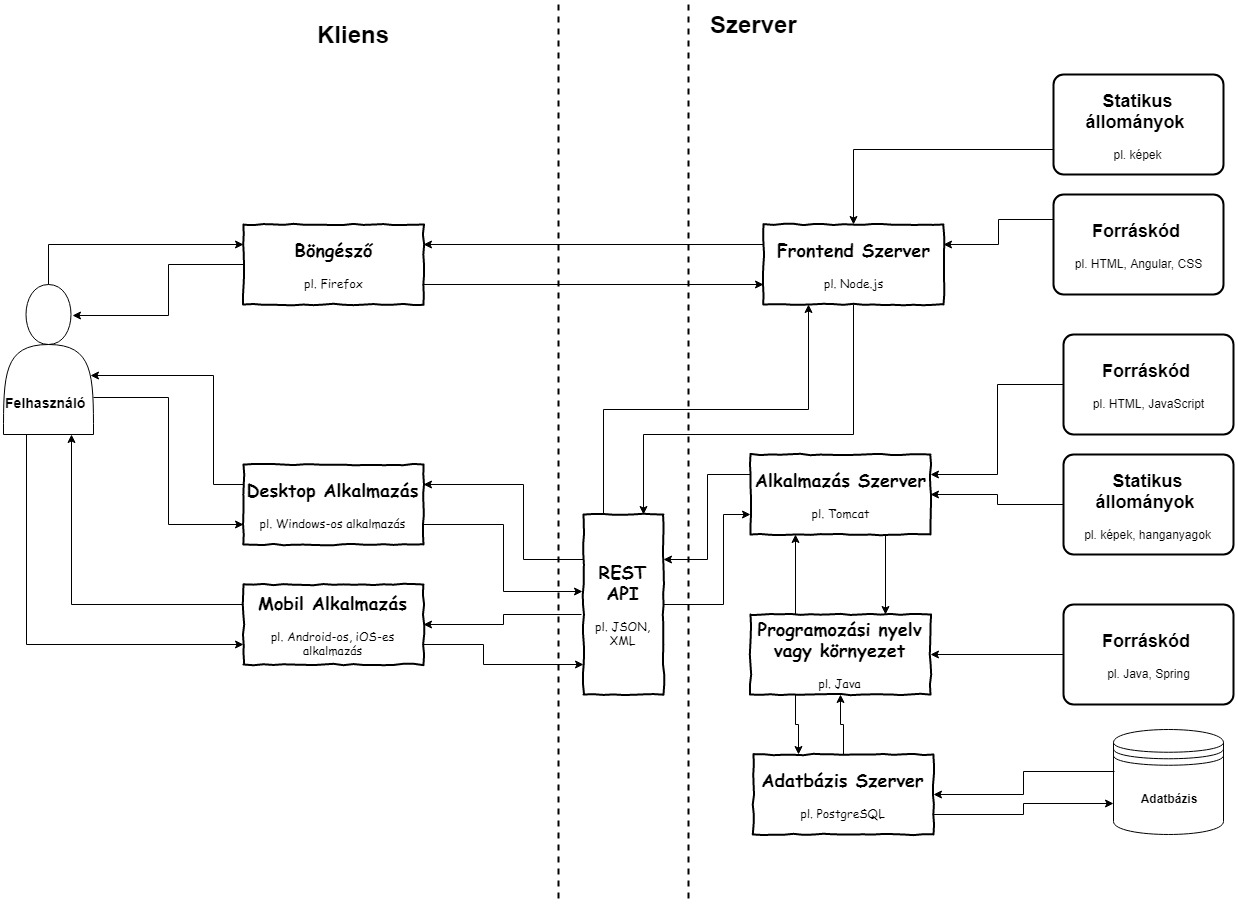
\includegraphics[scale=0.365]{kepek/architecture.jpg}
\caption{Szerver-kliens architektúra}
\label{fig:architecture}
\end{figure}

\subsection{Springről részletesebben, annotációk és bean-ek}

% Ez lehet, már az implementácsiós részhez kell majd.

Annotációk a Springben: Minden osztályban feltűnnek az annotációk. Melyek a keretrendszernek szóló üzenetek, ezek alapján tudja eldönteni a Spring, hogy miként bánjon az egyes osztályokkal, metódusokkal, adattagokkal.

Bean: Java komponensek, melyekből bármikor kérhetünk egy példányt a konténertől.

Konténer: A konténer tárolja és menedzseli a bean-ek - magyarul babok - élet ciklusait.

[9] \texttt{@Bean} Explicit módon adhatjuk meg vele a bean-eket a konténer számára.

\texttt{@Component} A komponensek is bean-ek csak ezeket automatikusan konfigurálja a keretrendszer. A Komponenseknek két válfaja van a \texttt{@Service} és a \texttt{@Repository}. A \texttt{@ComponentScan} annotációban megadott ösvényeket végigjárva keresi meg azokat az osztályokat, amelyeknek a definíciójában megtalálható valamelyik komponens típus.

\texttt{@Configuration} A bean leírások információforrása. Ilyen osztályokban konfiguráljuk a @Bean-eket.

\texttt{@EnableAutoConfiguration} Automatikus konfigurálás engedélyezése, ez az annotáció szól a Spring keretrendszernek, hogy amit tud azt állítson be magától, az alapértelmezett beállításokkal, és generálja le az ehhez kellő babokat.

\texttt{@ComponentScan} A konténernek megmondja, hogy melyik csomagokba vizsgálja meg, hogy bean-e vagy sem, ha bean akkor azt feljegyzi, hisz akkor úgy is kell kezelnie  a konténernek. Ha valamelyik osztály kér egy példányt egy bean-ből, akkor csak a konténerben regisztráltak közül tudunk kiosztani számára. Megadási módja, ha elég csak az a csomag amiben a @ComponentScan-nel annotált osztály elhelyezkedik, akkor nem kell paramétert megadni neki. Viszont, ha ez nem elég számunkra, akkor paraméterezni kell. A paraméterezés ilyen módon történik:
\begin{verbatim}
@ComponentScan(\{"hu.egyik", "hu.masik"\})
\end{verbatim}
tehát zárójelen belül, ha többet szeretnénk felsorolni, akkor kapcsos zárójelen belül, elemenként idézőjelek között felsorolva a csomagok nevét, és vesszővel elválasztva. Természetesen csak azokat az osztályokat találja meg, amelyik jelzi a konténer számára, hogy ő egy bean, pl.: @Component.

\texttt{@EnableAutoConfiguration}: Mindent állítson be magától a keretrendszer, amit csak tud.

\texttt{@Controller}: Controllerrel annotált osztály esetén @Requestmapping egy statikus file nevével tér vissza. (pl JSP vagy HTML file nevével.)

\texttt{@Service}: Jelzi a konténer számára, hogy ő a service réteghez tartozik, valamilyen számítások vagy transzformációk fognak végre hajtódni az adatokon amik ideérkeznek.

\texttt{@RestContoller}:
Jelzi a konténer felé, hogy innen érkezhetnek kérések, illetve itt tudjuk fogadni ezeket. És mint a neve is mutatja REST API segítségével. RestContoller elég nagy szabadság fokot biztosít, hisz szinte minden féle struktúrában adhatunk választ és fogadhatunk kérést, hisz ezeket értelmezni tudja. Tipikusan JSON-t fogunk használni, de lehetőség lenne akár XML, HTML választ is adni, a népszerűbb technológiákat kiemelve, de akár egyszerű konstansokat is. Tehát ennek az annotációnak a segítségével tudja a Spring, hogy ezzel az osztállyal lehet kommunikálni, ami azt jelenti, hogy tud küldeni és fogadni is adatot.

\texttt{@RequestMapping}:
A ReqestMapping annotáció segítségével megadhatjuk, hogy melyik csatornát figyelje a metódusunk, és ha a megadott csatornán jön valami, akkor meghívódik a hozzárendelt metódus.  A megadás módja \texttt{@ReqestMapping("/")}, tehát az annotáció után zárójelben, dupla idézőjelek között adjuk meg, hogy a honnan érkező kéréseket figyelje, a példában beállított a gyökércsatornán érkező kéréseket figyeli. (de ha /kiscica-t adok meg, akkor azokat fogja figyelni, ami azon a "kiscica" csatornán jön.)

\subsection{Spring Bean Scope}

A Spring Babok életciklusai.
Singleton: Csak egyetlen példány jön létre belőle. Ez a Springben az alapértelmezett, ha létrejön egy osztály az singleton lesz, ha másként nem rendelkezünk.(például: @RestContoller)
Prototype: Minden egyes alkalommal új példány készül.
Request: Mindenegyes HTTP lekérdezéssel új példányt készül belőle.
Session: Egy Session-höz kötjük a bean-t, a klasszikus példa erre a bevásárlókocsi a webáruházaknál, a kocsiba pakolt termékek addig maradnak amíg a felhasználó ki nem lép a böngészőből, vagy ki nem jelentkezik a weboldalról, így nem kell egy weblap frissítés után újra belepakolni a termékeket amiket meg szeretnénk vásárolni.

Az életciklusok megadásához a \texttt{@Scope} annotáció használatos, zárójelben idéző jelek között megadva a típust, például \texttt{@Scope("prototype")}.

\textit{@Autowired}
A Dependency Injection használatához van erre szükségünk. A keretrendszer aszerint injektálja a Bean-t amilyen a típusánál be van állítva, ha singleton akkor mindig ugyan azt az egyet adja át minden kérés esetén, ha prototype akkor minden egyes alakalommal új példányt ad át és így tovább.
Három fajta megadási mód létezik:
\begin{itemize}
\item Az adattag felett megadjuk és ez esetben, ha létrejön az objektum akkor a keretrendszer beleinjektálja az objektumot, amely ebben az esetben egy osztály szintű változó (static). Nehezen tesztelhető ez a fajta megadás.

\item A második mód a setter alapú megadási mód. Itt létrehozunk a változóhoz egy setter-t és a felett adjuk meg az annotációt.

\item Az utolsó verzió a konstruktor alapú, itt a konstruktor felett adjuk meg, a már jól ismert \texttt{@Autowired} annotációt.
\end{itemize}

\section{Az alkalmazás tervezése}

\begin{comment}{Az alább említett dolgok még a specifikációhoz tartoznak. A fejezet már elég ha csak azzal foglalkozik, hogy a specifikált dolgokat hogy lehet megvalósítani.}
\end{comment}

Az eddigiek alapján meg kell határozni, hogy miket szeretnénk, ha megvalósítana az alkalmazásunk, miben lesz más vagy jobb mint a többi a piacon fellelhető alkalmazás. Én igyekszem két új aspektust bevezetni, amelyeket ott nem, vagy nem egészen így alkalmaztak. Az egyik a fellépő alapú szemlélet. Szeretném, ha nemcsak a fesztiválról tudnánk meg többet, hanem az ott fellépő zenekarokról is érhetnénk el információkat. Ha nem ismerem őket, akkor rákattintva megtudhatok róluk pár információt, illetve az oldalra felvitt fesztiválok alapján a turné állomásokat. A másik aspektus a kulcsszavak bevezetése mint fesztivál, mint fellépő oldalon. Hasonlóval találkozhattunk egy-két általam is bemutatott oldalon. Amilyen paraméterek számításba jöhetnek: zenei stílusok, fesztivál stílusok, sátrazási lehetőség, kutyabarát. A divatos nevén a hashtag-ek. Adatbázis és program szinten stílusnak nevezem el, de talán ez egy kicsit tágabb fogalom.

\subsection{Alapfogalmak}

[22]A „hashtag” a metaadat egyik formája, amely egy szóból vagy kifejezésből áll, amely elé hash jelet (\#) tesznek. A hashtagek-et gyakran használják a közösségi hálókon, hogy azonosítsák, kategorizálják az érdeklődési köröket, „topikokat”, illetve megkönnyítsék a kulcsszavak szerinti kutatást.

[12] ER modell: Az ER modell, mint azt a neve (Entity Relationship) részben mutatja, három alapelemen nyugszik: az egyedeken (entity), az egyedek közötti kapcsolatokon (relation) és az egyedek tulajdonságain (attributes). Az ER modell kizárólag a valóság strukturális leírásán alapszik, megengedve bizonyos egyszerűbb integritási feltételeket is. Előnyei közé tartozik az egyszerűség, a szoros kapcsolat és a könnyű konvertálhatóság a relációs modell felé.
Az ER modell egyik lényeges tulajdonsága, hogy grafikus jelölésrendszert alkalmaz. A grafika, a szöveges leírástól eltérően sokkal kifejezőbb és lényegre törőbb az emberek számára, így kiválóan alkalmas a fontosabb fogalmak és kapcsolatok kiemelésére. A ma használatos ER modell teljes elemkészletének grafikai szimbólumait a következőkben adhatjuk meg:
\begin{itemize}
\item Egyed: egy a külvilág többi részétől egyértelműen megkülönböztethető dolog, objektum. 
\item Tulajdonság: az egyed egy meghatározott jellemzője.
\item Kapcsolat: az egyedek között fennálló viszonyt hordozza.
\end{itemize}

\subsection{ER modell}

ER-modellt használtam ahhoz, hogy szemléltessem az egyedek között fennálló relációkat és láthatóvá tegyem a megtervezett adatbázis architektúrát (\ref{fig:er}., {fig:usEr}. ábra).

\begin{figure}
\centering
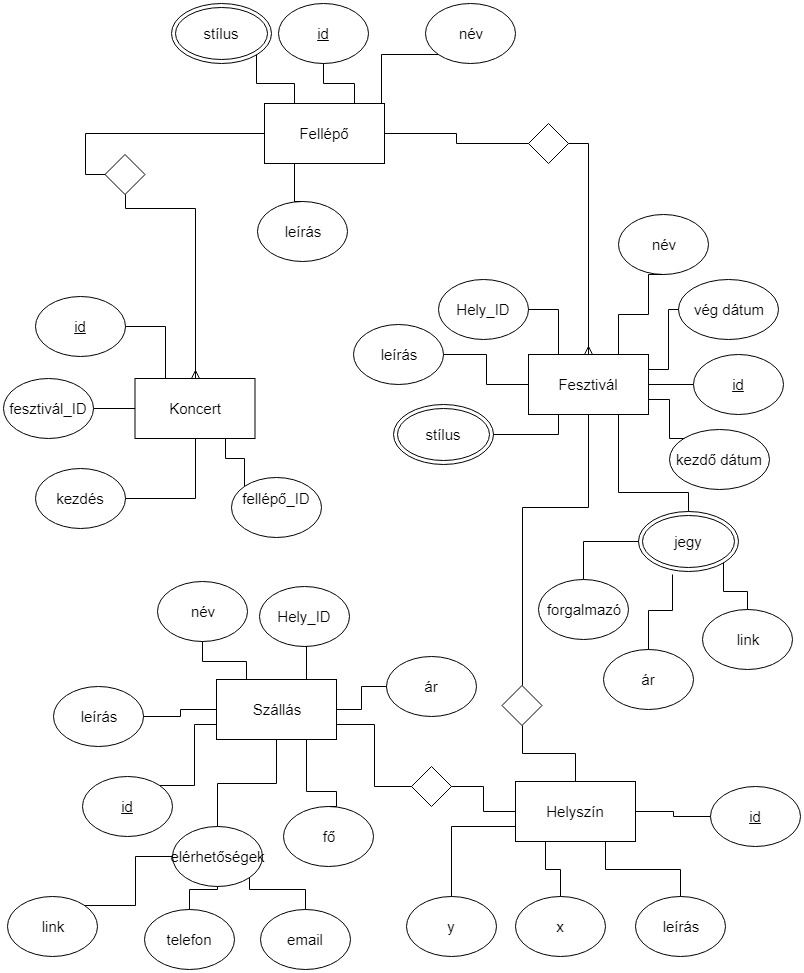
\includegraphics[scale=0.6]{kepek/er.jpg}
\caption{Az adatbázis ER diagramja}
\label{fig:er}
\end{figure}

\begin{figure}
\centering
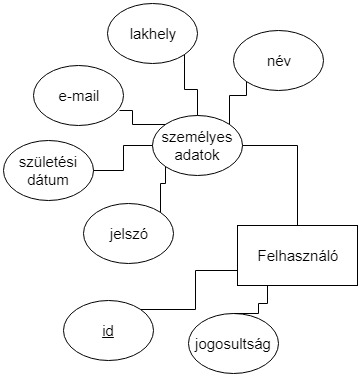
\includegraphics[scale=0.6]{kepek/userER.jpg}
\caption{Az adatbázis ER diagramja}
\label{fig:usEr}
\end{figure}

Lesz egy fellépő egyedünk, mivel zenei fesztiválokban gondolkodunk, így ezek zenekarok, vagy zenészek lesznek elsősorban. Egy fellépő több stílusban is játszhat, hisz ha egy zenekar népzenét játszik, az nem zárja ki, hogy ezt ötvözzék rockzenei motívumokkal. Sőt rengeteg előadó játszik több stílusban. A fellépőről tartunk számon egy rövid leírást. És elengedhetetlen, hogy az előadó nevét letároljuk. Az egyedi azonosítót pedig automatikusan generáltatjuk. 

Egy fesztiválkereső alkalmazást készítünk, így nem meglepő, hogy lesz egy fesztivál nevű entitásunk is. És talán ez lesz a legnagyobb komplexitású is. Minden fesztiválnak van egy neve, amely alapján a legkönnyebben azonosítják a rendszer felhasználói. Mivel egy ilyen esemény nem tart általában egész évben, ezért van egy kezdetét és végét jelző dátum. Erre a két időpontra azért is lesz szükségünk, hogy az érdeklő előre tudja  tervezni a programjait, és egyáltalán tudja, hogy nem-e ütközik valami más eseménnyel az általa kiválasztott fesztivál. Egy fesztiválnak is lehet több stílusa akár csak egy zenekarnak. Ahogy fentebb írtam itt nem csak a stílusok férnek bele, hanem egyéb jelzők is. Az ID generálást itt is az adatbázisra bízzuk. A leírás részt azoknak az információknak tartjuk fent, amelyekre nem készítettük fel a rendszerünk, és a marketing szövegeknek is kiváló helyet biztosít. A jegy a fejlesztés első fázisában nem lesz bevezetve, így csak egy hyperlink-et tartalmaz majd a forgalmazó weboldalára és nem külön egyedként, hanem egy oszlopként reprezentálódik az adatbázisban.

Koncert táblában két idegen kulcs lesz megtalálható, mivel ez a tábla kapcsolja össze a fellépőt a fesztivállal és ezáltal megtudjuk azt is, hogy milyen előadók vesznek részt az általunk preferált fesztiválon. Azt is megtudjuk nézni, hogy mikor kezdődik a számunkra érdekes előadás, mert egy kezdés nevű tulajdonságot is bevezettem. Lehetett volna tárolni azt is hogy mikor van vége. Alapvetően ez csak egy kapcsoló tábla, így nem szerettem volna túl bonyolítani, és ha valakit érdekel egy program, akkor úgyis kivárja a végét. Egyedi azonosítója ennek a táblának is lesz, amit itt is az adatbázisra bízunk.

Lesz egy helyszín nevű táblánk, amiben címek pozícióit lehet tárolni. Erre azért lesz szükségünk, hogy le tudjuk tárolni, hogy pontosan hol lesz az esemény, vagy a szállás. Természetesen itt is lesz egyedi azonosító minden rekordunkhoz. Ha az x és az y koordinátát tároljunk, akkor rengeteg dolgot ki tudunk váltani ezzel. Van a földnek egy egységes, minden tudományos intézmény által elfogadott geo koordináta rendszere. Ahol minden pozícióhoz tartozik egy hosszúsági és szélességi fok. Ezzel ki lehet váltani az hogy tároljuk a várost, az utcát, a házszámot, irányítószámot. De akár egy fesztivált szervezhetnek olyan helyre is, ahol ezek nincsenek is, akkor ahhoz egy másik struktúrát kellene bevezetni, amiben helyrajzi számot adunk át. És ha ezt a fesztivál szervező úgy kívánja megadni, hogy például az esemény egy adott csarnokban, vagy kulturális központban lesz, akkor megint egy újabb struktúra kerülne bevezetésre. Ha viszont csak a koordinátákat tároljuk, akkor ezeket valamilyen API-n keresztül, vagy előre mások által legyártott adatbázisból könnyen elérhetjük ezt egy koordináta rendszerbeli pont segítségével. Ha a legismertebb Google nevű cég által készített térkép alkalmazást nézzük, ott az egyes koordinátákhoz, nem csak címeket, de akár éttermeket, boltokat, cégeket és minden egyebet tárolhatunk, sőt ezeket még értékelni is lehet. Egy leírást is tárolunk, itt meg lehet adni extra információkat, hol és hogyan közelíthető meg a megadott pont, illetve amíg nem integráljuk az alkalmazást egy API-hoz vagy egyéb elérhető lehetőségek közül addig magát a címet is itt tároljuk.

A szállásokat is tároljuk az adatbázisunkban. Lesz egy fő nevű oszlopunk amely azt tárolja, hogy a szállás hány személyt képes befogadni, ez egy kisebb baráti társaság esetén lehet érdekes. Az ár tulajdonság egységárat tárol, tehát hogy mennyibe kerül egy éjszaka egy fő részére. Általában vannak egyedi konstrukciók, kedvezmények, de mivel mi nem foglalkozunk a foglalással, ezért csak irányárat mutatunk. Szolgáltatunk egy linket, ahol a foglalást el tudják végezni. Természetesen a szállás nevét is megadjuk. A címét az idegen kulcs segítségével könnyen megkaphatjuk. A leírásban minden egyebet tudunk rögzíteni. Az szállásadó elérhetőségeit is megadjuk az érdeklődök számára. A foglalási linken túl még egy telefonszámot és egy email címet is szolgáltat az alkalmazásunk.

Végül, de nem utolsósorban jönnek a felhasználóink, az alkalmazás regisztráció nélkül is teljes értékű alkalmazást nyújt egy keresni szándékozó felhasználó számára. A regisztrációra csak annak van szüksége, aki fel szeretne vinni az adatbázisba rekordokat. Itt több jogosultság is  felmerülhet. Fesztiválmenedzseri, aki a koncerteket, fesztiválokat viheti fel, ő felelős egy vagy több fesztivál menedzseléséért, a zenekarmenedzser, hasonló mint a fesztivál menedzser csak ő a fellépőkért felel. Adminisztrátori neki mindenhez van jogosultsága ami elérhető az alkalmazásból. Mi csak az adminisztrátori jogot fogjuk kiosztani, illetve az átlag felhasználót. A felhasználó személyes adatai közül az e-mail címét, nevét, születési dátumát és a lakhelyét, valamint a jelszavát tároljuk, amit valamilyen hasító algoritmuson lefuttathatunk előtte. Mint mindig itt is az adatbázisunk generálja az azonosítót.

Az egyedek között fent álló relációk a következőek:
\begin{itemize}
\item A fellépő egy-több kapcsolatban áll a koncerttel. Hiszen egy fellépő több koncerten is felléphet, de egy koncerten csak egy fellépő szokott fellépni. Persze van rá példa, hogy van vendég előadó, de ezek az extrém esetek, amúgy is gyakran meglepetések.
\item A fesztivál és a koncert között is egy-több kapcsolat van. Egyértelműen megállapítható az, hogy egy koncert csak egy fesztiválon lehet megrendezve - hasonló lehet máshol is, de egy fesztiválon több koncert is szokott lenni.
\item A fesztivál és a helyszín között egy-egy kapcsolat áll fent, habár a helyszín akár lehet egy település is. Egy fesztiválhoz egy helyszín tartozhat, és egy helyszínen akár több fesztivál is megszervezhető, de a redundancia elhanyagolható volta miatt elég lesz számunkra az egy-egy kapcsolat. Hisz egy fesztivál terület nem egy pont, hanem pontok halmaza. Lehetséges, hogy ugyanahhoz a helyszínhez több különböző pont is tartozik a térképen, így a redundancia tovább csökken.
\item  A helyszín és a szállás között egy-egy kapcsolat van, hiszen egy szálláshoz csak egy cím tartozhat.
\item A stílusok vagy metaadatok és a előadók között több-több kapcsolat van, de túl sok erőforrás pazarlásnak tartottam egy kapcsoló táblát bevezetni egy stílus miatt amiben semmi más nem tárolódik. Ezzel kapcsolatban több megoldást is számba vettem, ezek közül néhány: JSON vagy valamilyen no-SQL-ben eltárolom, és nem hozok létre a számára új táblát. Egy másik lehetőség egy saját struktúrának a bevezetése, például kettős keresztekkel elválasztva, és ez esetben sem lett volna új táblára szükségünk. Ezek a megoldások valamennyit gyorsíthattak is volna a megoldáson, de természetesen ezt tesztelés után lehetne eldönteni. Az egy-több kapcsolat megvalósításnál maradtam.
\item Az előzőhöz hasonlóan a fesztiválstílusok és a fesztivál között is ilyen a kapcsolat.
\end{itemize}

\subsection{Konkrét funkciók}

\begin{comment}{Ezt itt érdemes részletesebben kifejteni, vagy specifikációs jelleggel, vagy pedig már a konkrét implementációt emlegetve.}
\end{comment}

Lekérdezések: % a címeket formázni. 
\begin{itemize}
\item Összes stílust visszaadó funkció, amely értékkészletből könnyebben tud választani, ha esetleg nem jutna eszébe, vagy nem gondolna az esetleges kategóriákra.
\item Az összes fesztivált visszaadó funkció, amely mindezt a kezdés időpontja szerint adja vissza. Ez az alapértelmezett, ha a fesztiválok menüpontra kattintunk.
\item Fesztivál visszaadás Id alapján. Egy fesztivált kiválasztunk, a részleteit, illetve a programját az azonosítója alapján kapjuk vissza. 
\item Kiválasztott stílus alapján megkapjuk azon fesztiválok listáját, amelyek a kategória alá tartoznak.
\item Fesztiválok település alapján, ez megvalósulhat API alapján, illetve amíg az nincs addig az egyed leírásából kinyerhető lesz a helyszín. 
\item Fesztivál koordinátáitól 10 km távolságra eső szállások. Akár lehet megadott távolság is, de a szállás keresést nem szeretném a felhasználóra bízni. Hanem a fesztivál kiválasztásakor ajánl a rendszer a fesztiválhoz közeli szállásokat. De akár ez megvalósulhat önálló funkcióként is, ahol megadott koordinátától, megadott távolságra lévő szállásokat tudunk megkeresni, itt a megadott koordináta lehet a fesztivál, a felhasználó meg kiválaszthatja, hogy milyen távolságon belül keres szállást.
\item Fesztiválok keresése két dátum közötti intervallumban, ha a felhasználó az egyiket üresen hagyja, arra is fel kell készíteni a rendszert.
\item Fesztiválok fellépő alapján listázzuk ki az összes olyan fesztivált, amelyiken fellép a kiválasztott fellépő.
\item Koncertek fellépő alapján, hasonló mint az előző, csak itt a pontos időpont is kiderül, hogy mikor lesz a fellépés, illetve a koncert specifikus részletek. %lehet bevezetek egy új adattagot leírás néven a koncerthez.
\item Koncertek fesztivál alapján:  Kiválasztott fesztivál programja. itt érdemes lehet valamilyen rendezési elvet használni. Napokra bontani, betűrend szerint rendezni, vagy színpad szerint csoportosítani. % ehhez kell egy színpad adattag.
\item Fellépők listázása betűrendben.
\item Fellépők visszaadása név, vagy névrészlet alapján.
\item Az összes olyan fellépő visszaadása amelyiknek a stílusa megegyezik a lekért stílussal. A kérés érkezhet egy hashtag-re kattintásból, de lehetőség lesz stílusra is keresni.
\item Lakóhelytől, vagy egy a felhasználótól bekért pozíciótól megadott távolságon belüli fesztiválok.
\end{itemize}

Új elemek hozzáadása:
\begin{itemize}
\item Szállások felvitele pozíciójával együtt.
\item Fesztivál felvitele pozíciójával és stílusaival együtt.
\item Koncert felvitele, ami valójában egy fellépő és egy fesztivál összekapcsolása.
\item Zenekar felvitele a stílusaival együtt.
\item Új további stílusok hozzáadása zenekarhoz. Itt esetleg bevezetésre kerülhet egy érték készlet is.
\item Plusz stílusok hozzáadása egy fesztiválhoz.
\end{itemize}

 Elemek törlése:
\begin{itemize}
\item Stílusok törlése. Vonatkozik mind a zenei, mind a fesztivál stílusokra. 
\item Koncert törlése.
\item Fesztivál törlése, itt figyelni kell arra, hogy a törlés előtt fel kell szabadítani minden olyan erőforrást ami függ tőle. Tehát törölni kell a koncertjeit, stílusait és a koncert helyszínt is.
\item Fellépő törlése nem jellemző, ha mégis kell akkor azt meg lehet oldani adatbázis szinten is.
\item Szállás törlésénél is figyelni kell, hogy a hozzátartozó helyszínt is törölni kell vele együtt.
\item Amelyik fesztivál és koncert elmúlt, tehát a befejezés dátumán már az aktuális naptári idő  túlhaladt, azt archiválni kell. Erre a funkcióra elég egy triggert írni. Archiválás megvalósítása megoldható úgy, hogy átmozgatjuk egy másik táblába, vagy egy új változó bevezetésével, és azt hogy elérhető-e elég igazról hamisra állítani. Esetleg a mindent vissza adó függvény csak azt adja vissza amelynek a befejező dátuma nagyobb mint az aktuális dátum.
\end{itemize}
Módosítások:
\begin{itemize}
\item Helyszín módosítása.
\item Stílust nem érdemes módosítani. Jobb megoldás a törölés, és helyette egy másikat felvinni.
\item Fesztivál módosítása Ezen belül meghívható a helyszín módosítás és itt hajtható végre a stílusok törlés vagy új felvitele.
\item Zenekar módosítása. A fesztivál törléséhez hasonlóan itt lehet a stílus törlését is elérni a felületen.
\item Koncert módosítása.
\item Szállás módosítása, beleértve a pozíciójának a módosítását. 
\end{itemize}

\begin{comment}{Az egyes hibalehetőségeket is sorra kellene majd venni!}
\end{comment}

\begin{comment}{Meg kellene nézni, hogy hogy lehetne esetleg még jobban csoportosítani a listaelemekben említett dolgokat, és inkább alpontokba rendezni alcímekkel együtt.}
\end{comment}

\subsection{Struktúra}
